\section{Task 3}
\subsection{Matrix 2-norm: overview and comparison}

The matrix 2-norm (spectral norm) is defined as the largest singular value of \( A \). It equals the square root of the largest eigenvalue of \( A^T A \), allowing the distribution of matrix values to be assessed.

Our algorithm computes this norm by finding roots of the matrix's characteristic polynomial. This approach is sensitive to numerical errors, particularly when eigenvalues are close together. Polynomial-root operations can produce unwanted effects, including complex error values caused by rounding or numerical instability.

The \textit{power method} can normally be used to compute the matrix 2-norm. This iterative technique provides a stable approximation of the largest eigenvalue. Its steps are:
\begin{enumerate}
    \item Start with a vector \( v_0 \) of arbitrary values.
    \item At each iteration, compute \( v_{k+1} = Av_k \) and normalize the resulting vector.
    \item Repeat until the iterations converge to the eigenvalue with the largest absolute value.
\end{enumerate}
This method is more stable than operations on the characteristic polynomial because it avoids rounding-error problems and does not require finding polynomial roots.

\subsection{Results and conclusions:}

Comparing our \( \text{norm2} \) function with Octave's built-in \( \text{norm} \), we observe discrepancies due to numerical errors. Our implementation is more sensitive to errors in characteristic-polynomial roots, particularly for matrices with similar eigenvalues. Large diagonal values can also cause rounding errors because arithmetic precision is limited.

The following plot illustrates errors in our implementation.

\centering 
\begin{minipage}{0.6\textwidth}
    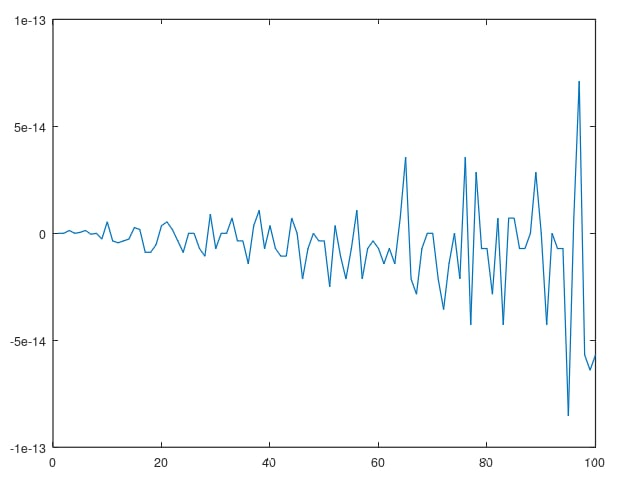
\includegraphics[width=\textwidth]{figures/zadanie3_error.jpg}
\end{minipage}

\textbf{Conclusions:}
\begin{itemize}
    \item Error values fluctuate substantially. The algorithm is numerically unstable.
\end{itemize}
